\documentclass[a4paper]{article}
\usepackage[utf8]{inputenc}
\usepackage[russian]{babel}
\usepackage[T2]{fontenc}
\usepackage[warn]{mathtext}
\usepackage{graphicx}
\usepackage{amsmath}
\usepackage{floatflt}
\usepackage[left=20mm, top=20mm, right=20mm, bottom=20mm, footskip=10mm]{geometry}


\graphicspath{ {images/} }
\usepackage{multicol}
\setlength{\columnsep}{2cm}


\begin{document}

\begin{titlepage}
	\centering
	\vspace{5cm}
	{\scshape\LARGE Московский физико-технический институт \par}
	\vspace{5cm}

	{\huge\bfseries Термоэлектронный диод \par}
	\vspace{1cm}
	{\scshape\Large Лабораторная работа по курсу <<Вакуумная электроника>>\par}
	\vspace{1cm}
	\vfill
\begin{flushright}
	{\large выполнила студентка 653 группы ФФКЭ}\par
	\vspace{0.3cm}
	{\LARGE Карпова Татьяна Кирилловна} \par

	
\end{flushright}
	

	\vfill

% Bottom of the page
	Долгопрудный, 2018 г.
\end{titlepage}

\section{Цель работы}
\begin{itemize}
    \item Практическое изучение явления термоэлектронной эмиссии и процессов токопрохождения в вакууме;
    \item Изготовление вакуумного диода;
    \item Исследование некоторых характеристик диода;
    \item Проверка справедливости законов Ричардсона-Дешмана и Чайлда-Ленгмюра.
\end{itemize}

\section{Лабораторная установка}
Схема лабораторной установки для исследования характеристик термоэлектронного диода приведена на рис. 1.

\begin{figure}[h]
    \centering
    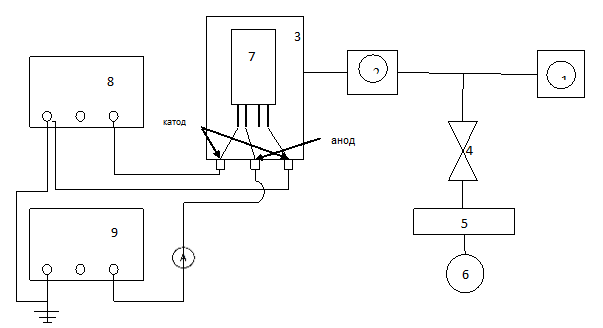
\includegraphics[width=13cm]{setup.PNG}
    \caption{Принципиальная схема лабораторной установки}
    \label{fig:vac}
\end{figure}
\begin{enumerate}
    \item Форвакуумный насос
\item Турбомолекулярный насос
\item Вакуумная камера
\item Клапан с электрическим управлением
\item Измерительная насадка
\item Фильтр входящего воздуха
\item Диод
\item Источник питания HY 3010E
\item Вольтметр GPR-30H100
\end{enumerate}

\section{Выполнение работы}
\begin{enumerate}
    \item Проведём прогревание катода, снимем зависимость тока накала от напряжения накала. График зависимости приведён на рисунке 2.
    


\item Рассчитаем сопротивление диода по формуле 
\begin{center}
    $R = \frac{U}{I}$,
\end{center}

подаваемую мощность - по формуле

\begin{center}
    $P = U I$
\end{center}

Построим график зависимости сопротивления катода от приложенной мощности (рисунок 3)



\item Построим графики зависимости температуры катода от тока накала.  \par
Для графика, построенного на основании изменения сопротивления катода, температуру будем вычислять по формуле, полученной в результате преобразований:
\begin{center}
   $ \rho_T = \rho_0 (1 + \alpha T) $, \\
   $T = \frac{\rho_T - \rho_0}/{\alpha \rho_0}$
\end{center}
где $\alpha = 9,29 * 10^{-3}$ - коэффициент температурной зависимости электрического сопротивления, $\rho_0$ - удельное сопротивление материала катода при $0^{\circ}$. \par

Для графика, построенного на основании расчётов с использованием уравнения энергетического баланса, используем формулу 
\begin{center}
    $T_k = (\frac{P}{\varepsilon S \sigma})^{1/4}$,
\end{center}
где $S$ - площадь эмитирующей поверхности, $\varepsilon = 0.032$ - степень черноты материала катода, $\sigma = 5.67*10^{-8}$ Дж/(с*м$^2$*K$^4$). \par
На одном графике представим эти зависимости, их характеры совпадают.



\item Построим графики зависимости анодного тока от анодного напряжения пи различных значениях тока накала в координатах $lg(I_A)$ от $lg(U_A)$



\item По этим данным определим первеанс диода $g$. Зная, что $I_a = gV_A^{3/2}$ и имея зависимости $\lg(I_A) = k \lg(V_A) + b$, получим
\begin{center}
    $g = 10^{\frac{3b}{2k}}$
\end{center}

Определим первеанс по разным данным тока накала диода и сравним значения с расчётным, вычисляющимся по формуле

\begin{center}
    $g = 2.33*10^{-6} \frac{S_c}{R_a ^2} = 88*10^{-6}$,
\end{center}
где $S_c$ - площадь поверхности катода, $R_a$ - радиус анода. \par

Также вычислим отношение заряда электрона к его массе по формуле

\begin{center}
   $e/m = \frac{81}{8}(g\frac{R_a}{L_a})^2$
\end{center}

Наконец, эффективность катода вычислим по формуле
\begin{center}
    $\eta = \frac{I}{P}$
\end{center}

    \begin{table}[h]
    \centering
    \begin{center}
    \caption{Значения первеанса по разным опытам}
    \end{center}
    \vspace{0.1cm}
    \label{tab:my_label}
    \begin{tabular}{ |p{1cm}|p{1cm}|p{1cm}|p{1cm}|p{2cm}|p{2cm}|p{2cm}|}
 \hline
 $I$, А & $U$, B & k & b & g & e/m, $10^{-9}$ & $\eta$, \% \\
 \hline
 \hline
2.5 & 3.8 & 0.5 & -3.85 & 2.37*$10^{-10}$ & 9.2 & 26.3\\
 \hline
2.6 & 4.2 & 0.78 & -3.65 & 9.56*$10^{-8}$ & 24.0 & 23.8\\
 \hline
2.7 & 4.5 & 1.07 & -4.1 & 1.79*$10^{-6}$ & 154.6 & 22.2\\
 \hline
2.8 & 4.9 & 1.27 & -4 & 18.86*$10^{-6}$ & 348.7 & 20.4 \\
 \hline
2.9 & 5.2 & 1.24 & -3.85 & 22.02*$10^{-6}$ & 72.7 & 19.2\\
 \hline
3.0 & 5.5 & 1.42 & -4.2 & 67.21*$10^{-6}$ & 45.8 & 18.2\\
 \hline 

\end{tabular}
\end{table}

\item Построим зависимость анодного тока от тока накала при напряжении V = 110 B

\end{enumerate}

\section{Вывод}

В ходе лабораторной работы
\begin{enumerate}
    \item Были получены представления о структуре элементарного диода

    \item Были изучены следующие характеристики диода: вольт-амперная характеристика, первеанс и его эффективность;

    \item Были проверены закономерности ВАХ диода: при больших токах накала - справедливо уравнение Чайлда-Ленгмюра, а при насыщении – уравнение Ричардсона-Дэшмана;

    \item Была рассчитана температура катода, исходя из трёх разных позиций: с точки зрения сопротивления катода, с точки зрения уравнения энергетического баланса, с точки зрения закона Ричардсона-Дэжзшмана;

\end{enumerate}

\section{Список литературы}
\begin{enumerate}
    \item Батурин А.С., Кириченко Л.А., Коновалов Н.Д. и др. Под ред. Шешина Е.П. Эмиссионная электроника в примерах и задачах: учебное пособие / --М.:МФТИ, 2002 - 193 с. 
    \item Батурин А.С., Стариков П.А., Шешин Е.П. Термоэлектронный диод: лабораторная работа по курсу Вакуумная электроника /--М.:МФТИ, 2008 - 43 с.
\end{enumerate}

\newpage

\begin{figure}[h]
\begin{center}
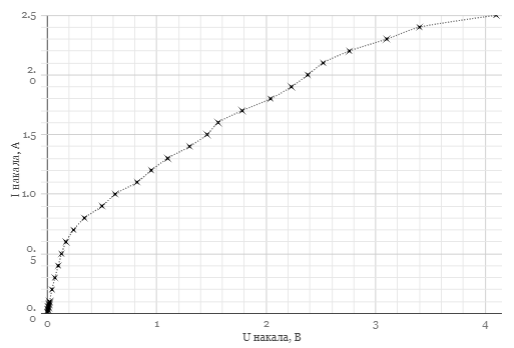
\includegraphics[width=13cm]{fig1.PNG}
\caption{Зависимость тока накала от напряжения накала}
\label{ris:experimoriginal} %% метка рисунка для ссылки на него
\end{center}
\end{figure}

\begin{figure}[h]
\begin{center}
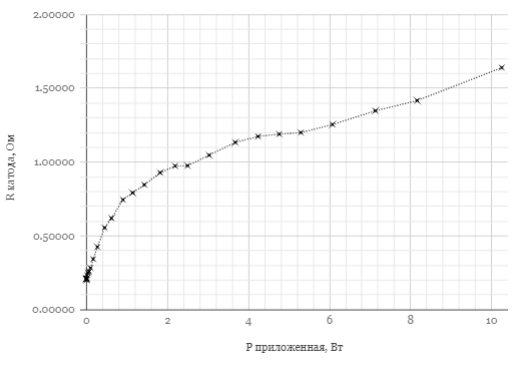
\includegraphics[width=13cm]{fig2.PNG}
\caption{Зависимость сопротивления катода от приложенной мощности}
\label{ris:experimoriginal} %% метка рисунка для ссылки на него
\end{center}
\end{figure}

\begin{figure}[h]
\begin{center}
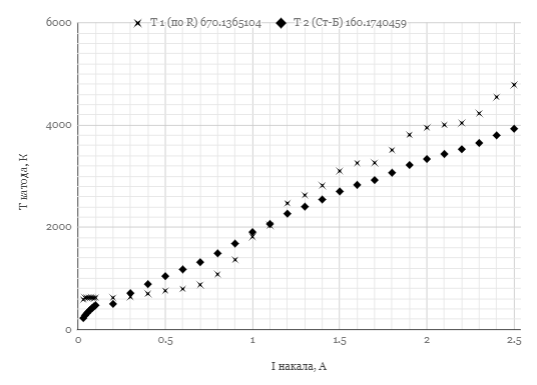
\includegraphics[width=13cm]{fig3.PNG}
\caption{Зависимость температуры катода от тока накала: расчёт по измерению сопротивления и по уравнению Стефана-Больцмана}
\label{ris:experimoriginal} %% метка рисунка для ссылки на него
\end{center}
\end{figure}

\begin{figure}[h]
\begin{center}
\begin{minipage}[h]{0.45\linewidth}
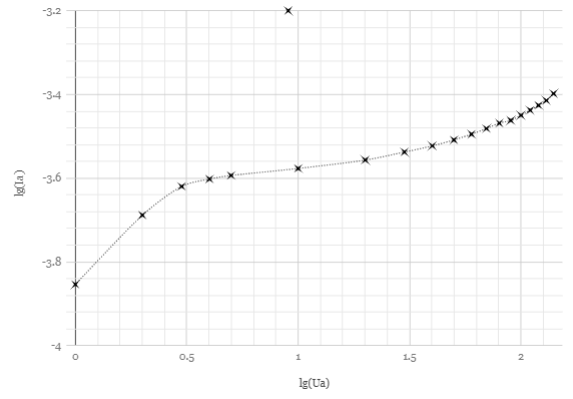
\includegraphics[width=1\linewidth]{2_5.PNG}
\caption{Зависимость $lg(I_A)$ от $lg(V_A)$ при токе накала 2.5 А, напряжении накала 3.8 B} %% подпись к рисунку\label{ris:experimoriginal} %% метка рисунка для ссылки на него
\end{minipage}
\hfill 
\begin{minipage}[h]{0.45\linewidth}
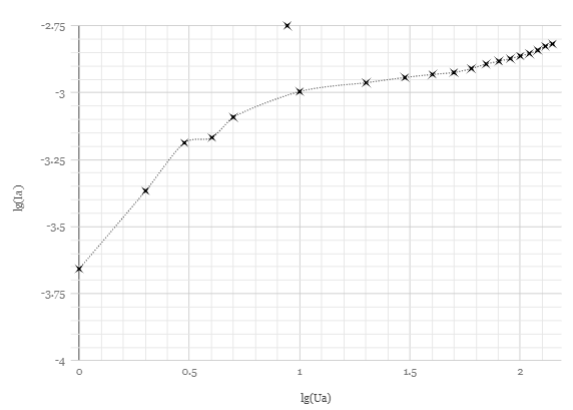
\includegraphics[width=1\linewidth]{2_6.PNG}
\caption{Зависимость $lg(I_A)$ от $lg(V_A)$ при токе накала 2.6 А, напряжении накала 4.2 B }
\label{ris:experimcoded}
\end{minipage}
\end{center}
\end{figure}

\begin{figure}[h]
\begin{center}
\begin{minipage}[h]{0.45\linewidth}
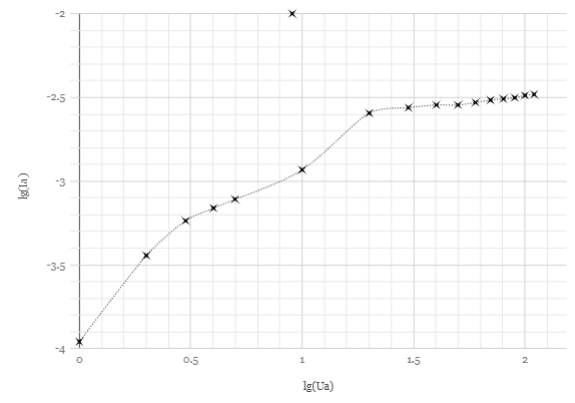
\includegraphics[width=1\linewidth]{2_7.PNG}
\caption{Зависимость $lg(I_A)$ от $lg(V_A)$ при токе накала 2.7 А, напряжении накала 4.5 B} %% подпись к рисунку\label{ris:experimoriginal} %% метка рисунка для ссылки на него
\end{minipage}
\hfill 
\begin{minipage}[h]{0.45\linewidth}
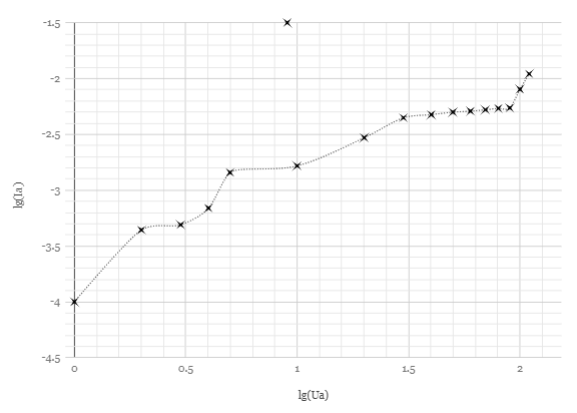
\includegraphics[width=1\linewidth]{2_8.PNG}
\caption{Зависимость $lg(I_A)$ от $lg(V_A)$ при токе накала 2.8 А, напряжении накала 4.9 B }
\label{ris:experimcoded}
\end{minipage}
\end{center}
\end{figure}

\begin{figure}[h]
\begin{center}
\begin{minipage}[h]{0.45\linewidth}
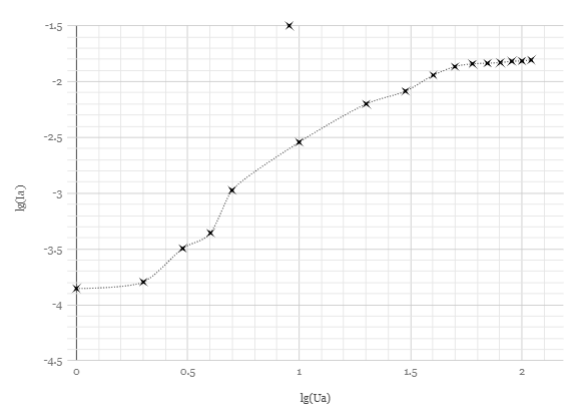
\includegraphics[width=1\linewidth]{2_9.PNG}
\caption{Зависимость $lg(I_A)$ от $lg(V_A)$ при токе накала 2.9 А, напряжении накала 5.2 B} %% подпись к рисунку\label{ris:experimoriginal} %% метка рисунка для ссылки на него
\end{minipage}
\hfill 
\begin{minipage}[h]{0.45\linewidth}
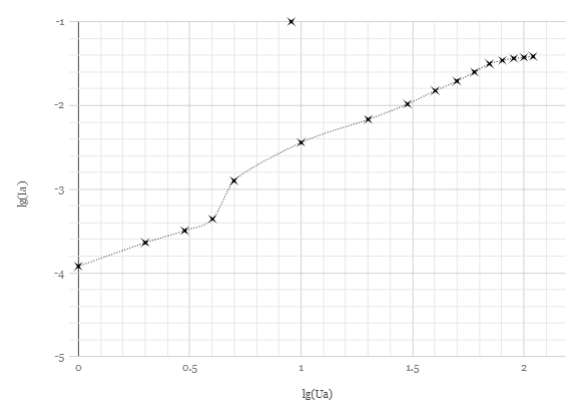
\includegraphics[width=1\linewidth]{3_0.PNG}
\caption{Зависимость $lg(I_A)$ от $lg(V_A)$ при токе накала 3.0 А, напряжении накала 5.5 B }
\label{ris:experimcoded}
\end{minipage}
\end{center}
\end{figure}

\begin{figure}[h]
\begin{center}
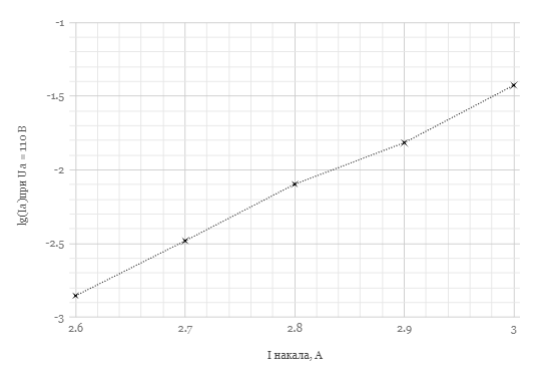
\includegraphics[width=13cm]{fig4.PNG}
\caption{Зависимость $lg(I_A)$ от тока накала при V = 110 B}
\label{ris:experimoriginal} %% метка рисунка для ссылки на него
\end{center}
\end{figure}

\end{document}
